\placelogofalse
\begin{frame}{Finite Element Analysis (FEA)}
\begin{columns}
\column{0.48\linewidth}
\centering
\begin{outline}
  \1 Numerically solve differential equations
  \1 Example uses:
  \2 Linear elasticity
  \2 Thermal transfer
  \2 Fluid flow
  \1 Geometric domains
  \1 Boundary Conditions
%  \1 Aid in design, testing, and validation
\end{outline}

\column{0.58\linewidth}
\centering
\begin{center}

\shadowimage[width=2.8cm]{wiki_car_example.png} 
\shadowimage[width=3.4cm]{crowbar_modal.png}

\shadowimage[width=3.5cm]{ship_example.png}
\shadowimage[width=2cm]{BLAST_example.png}

\end{center}
\end{columns}
\blfootnote{Images from \href{https://en.wikipedia.org/wiki/Finite_element_method}{Wikipedia},
  \href{https://www.intact-solutions.com/}{Intact Solutions},
\href{https://computing.llnl.gov/projects/blast/triple-point-shock-interaction}{LNLL}}
\end{frame}
\placelogotrue

\begin{frame}{Heat Sink Example}
  \centering
  \begin{center}
    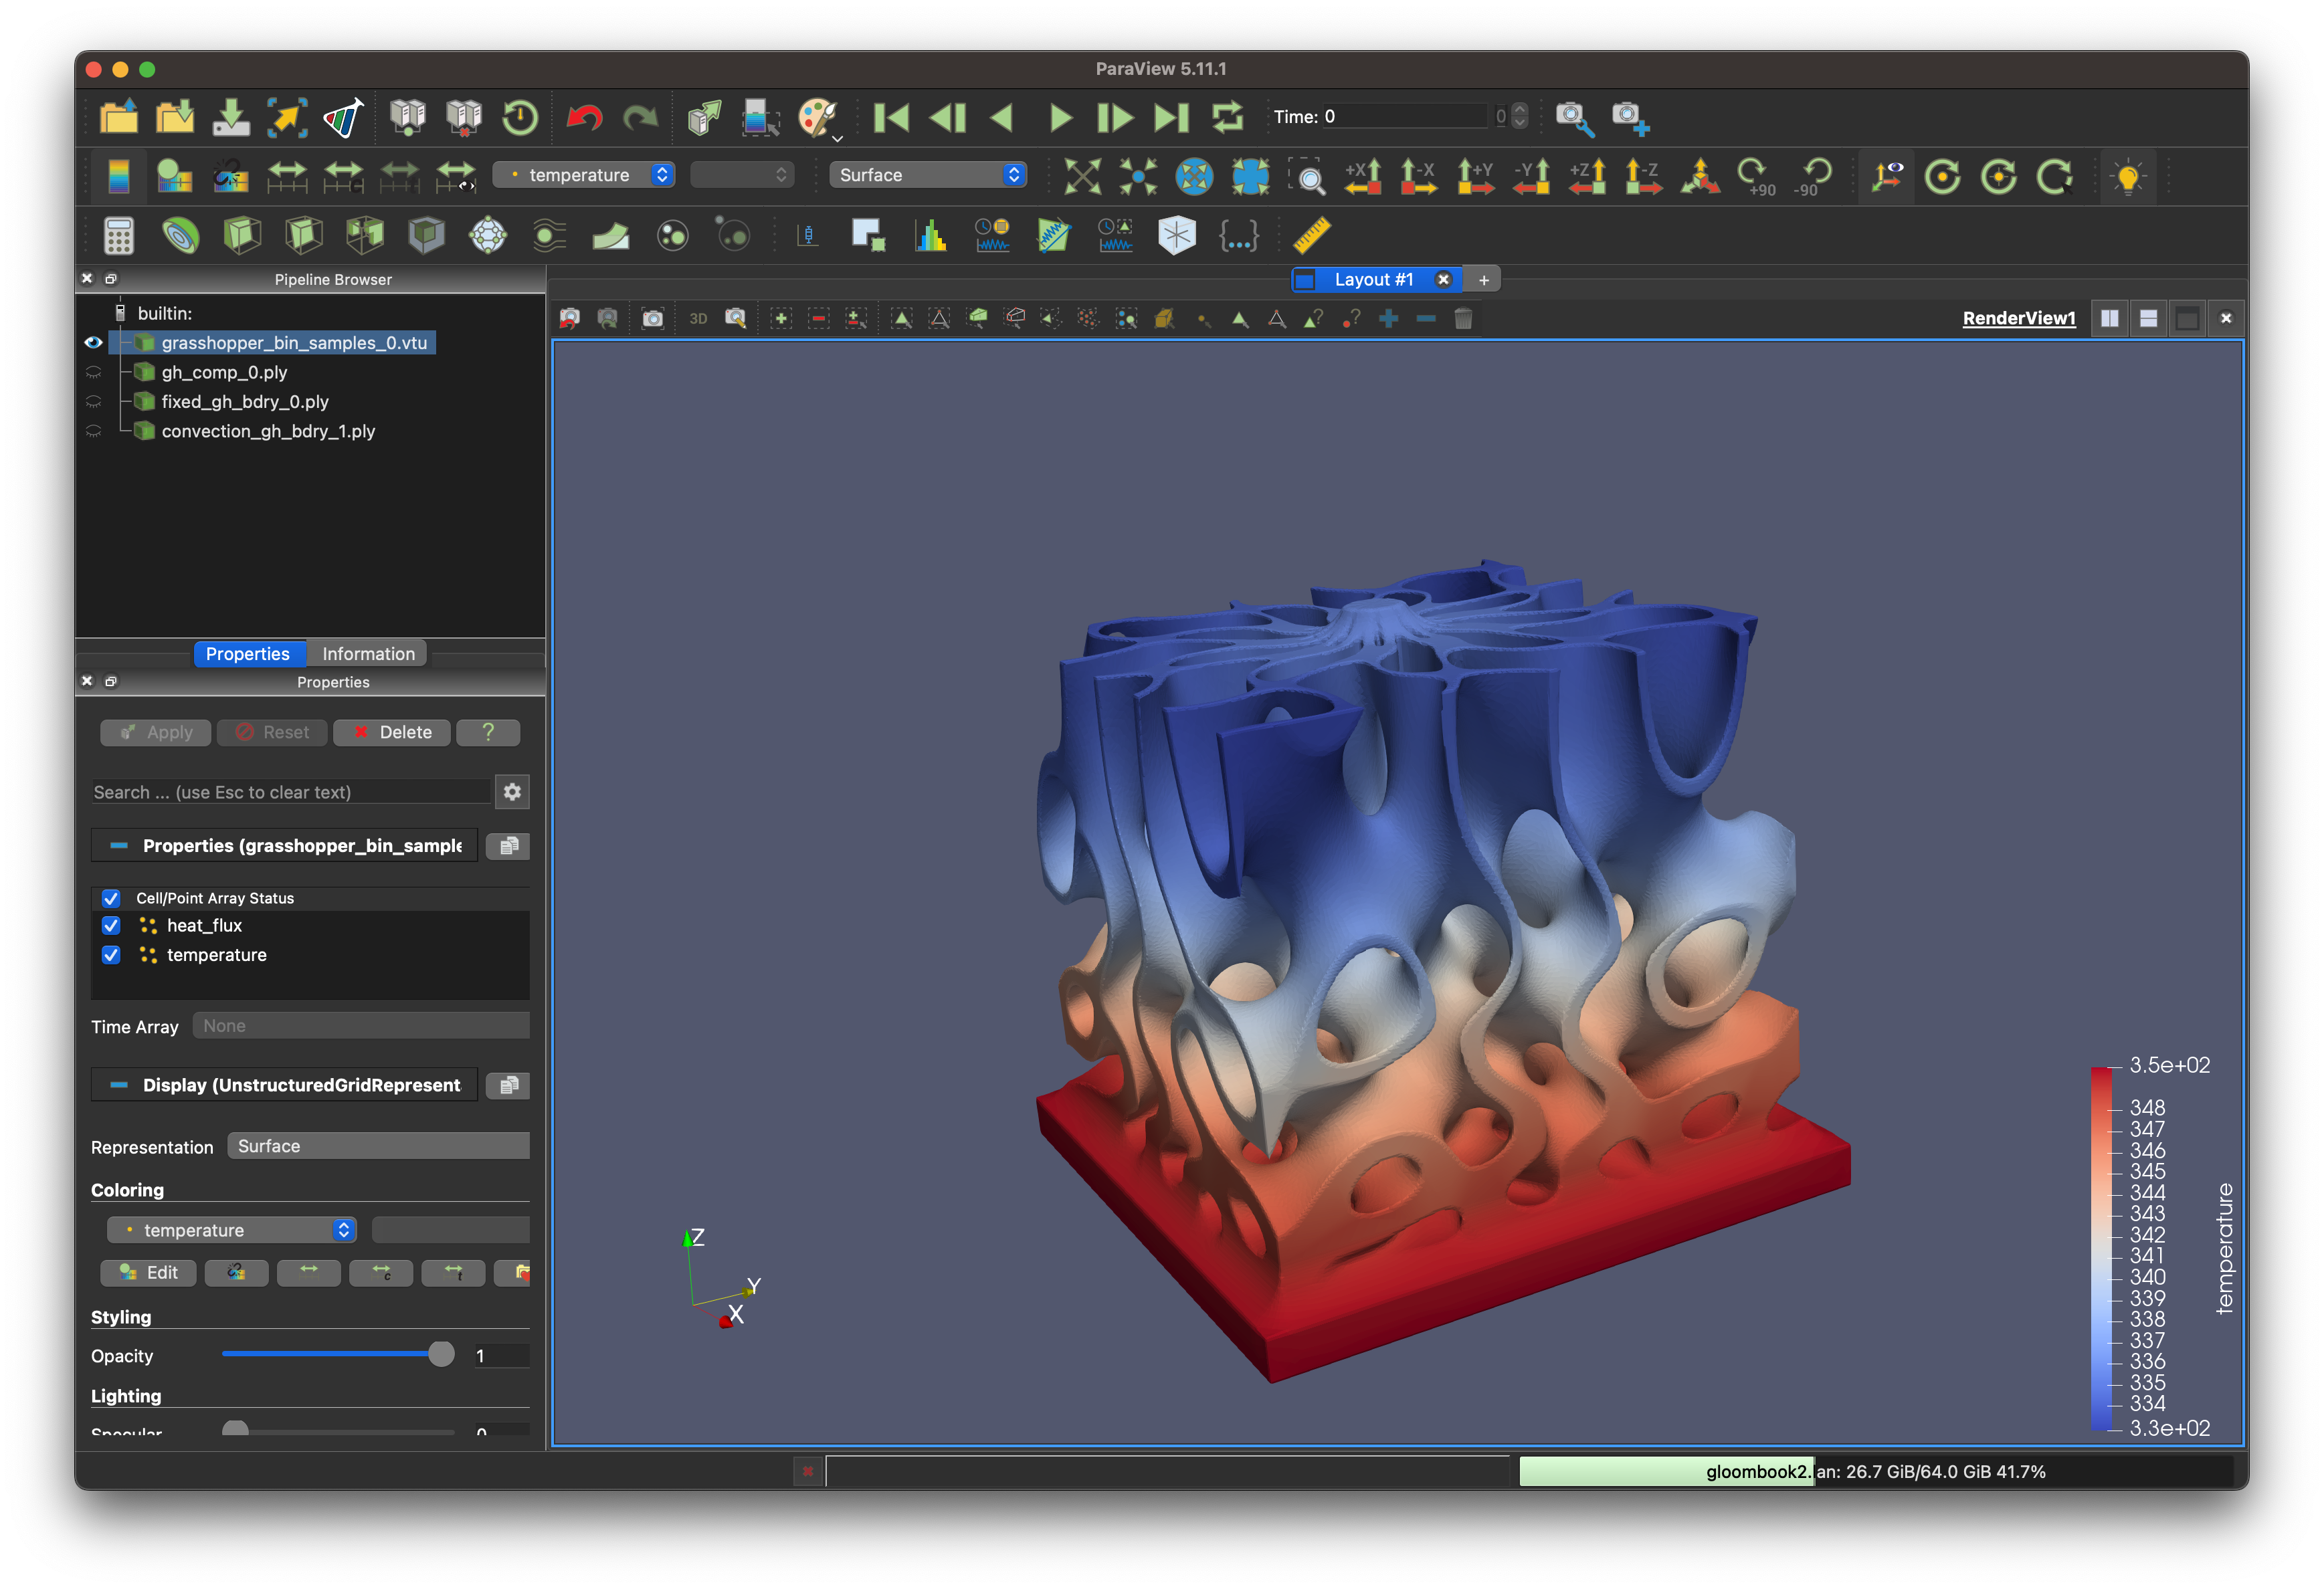
\includegraphics[width=0.7\linewidth]{heat_sink_example.png}
  \end{center}
\end{frame}

\begin{frame}{Bracket Example}
  \centering
  \begin{center}
    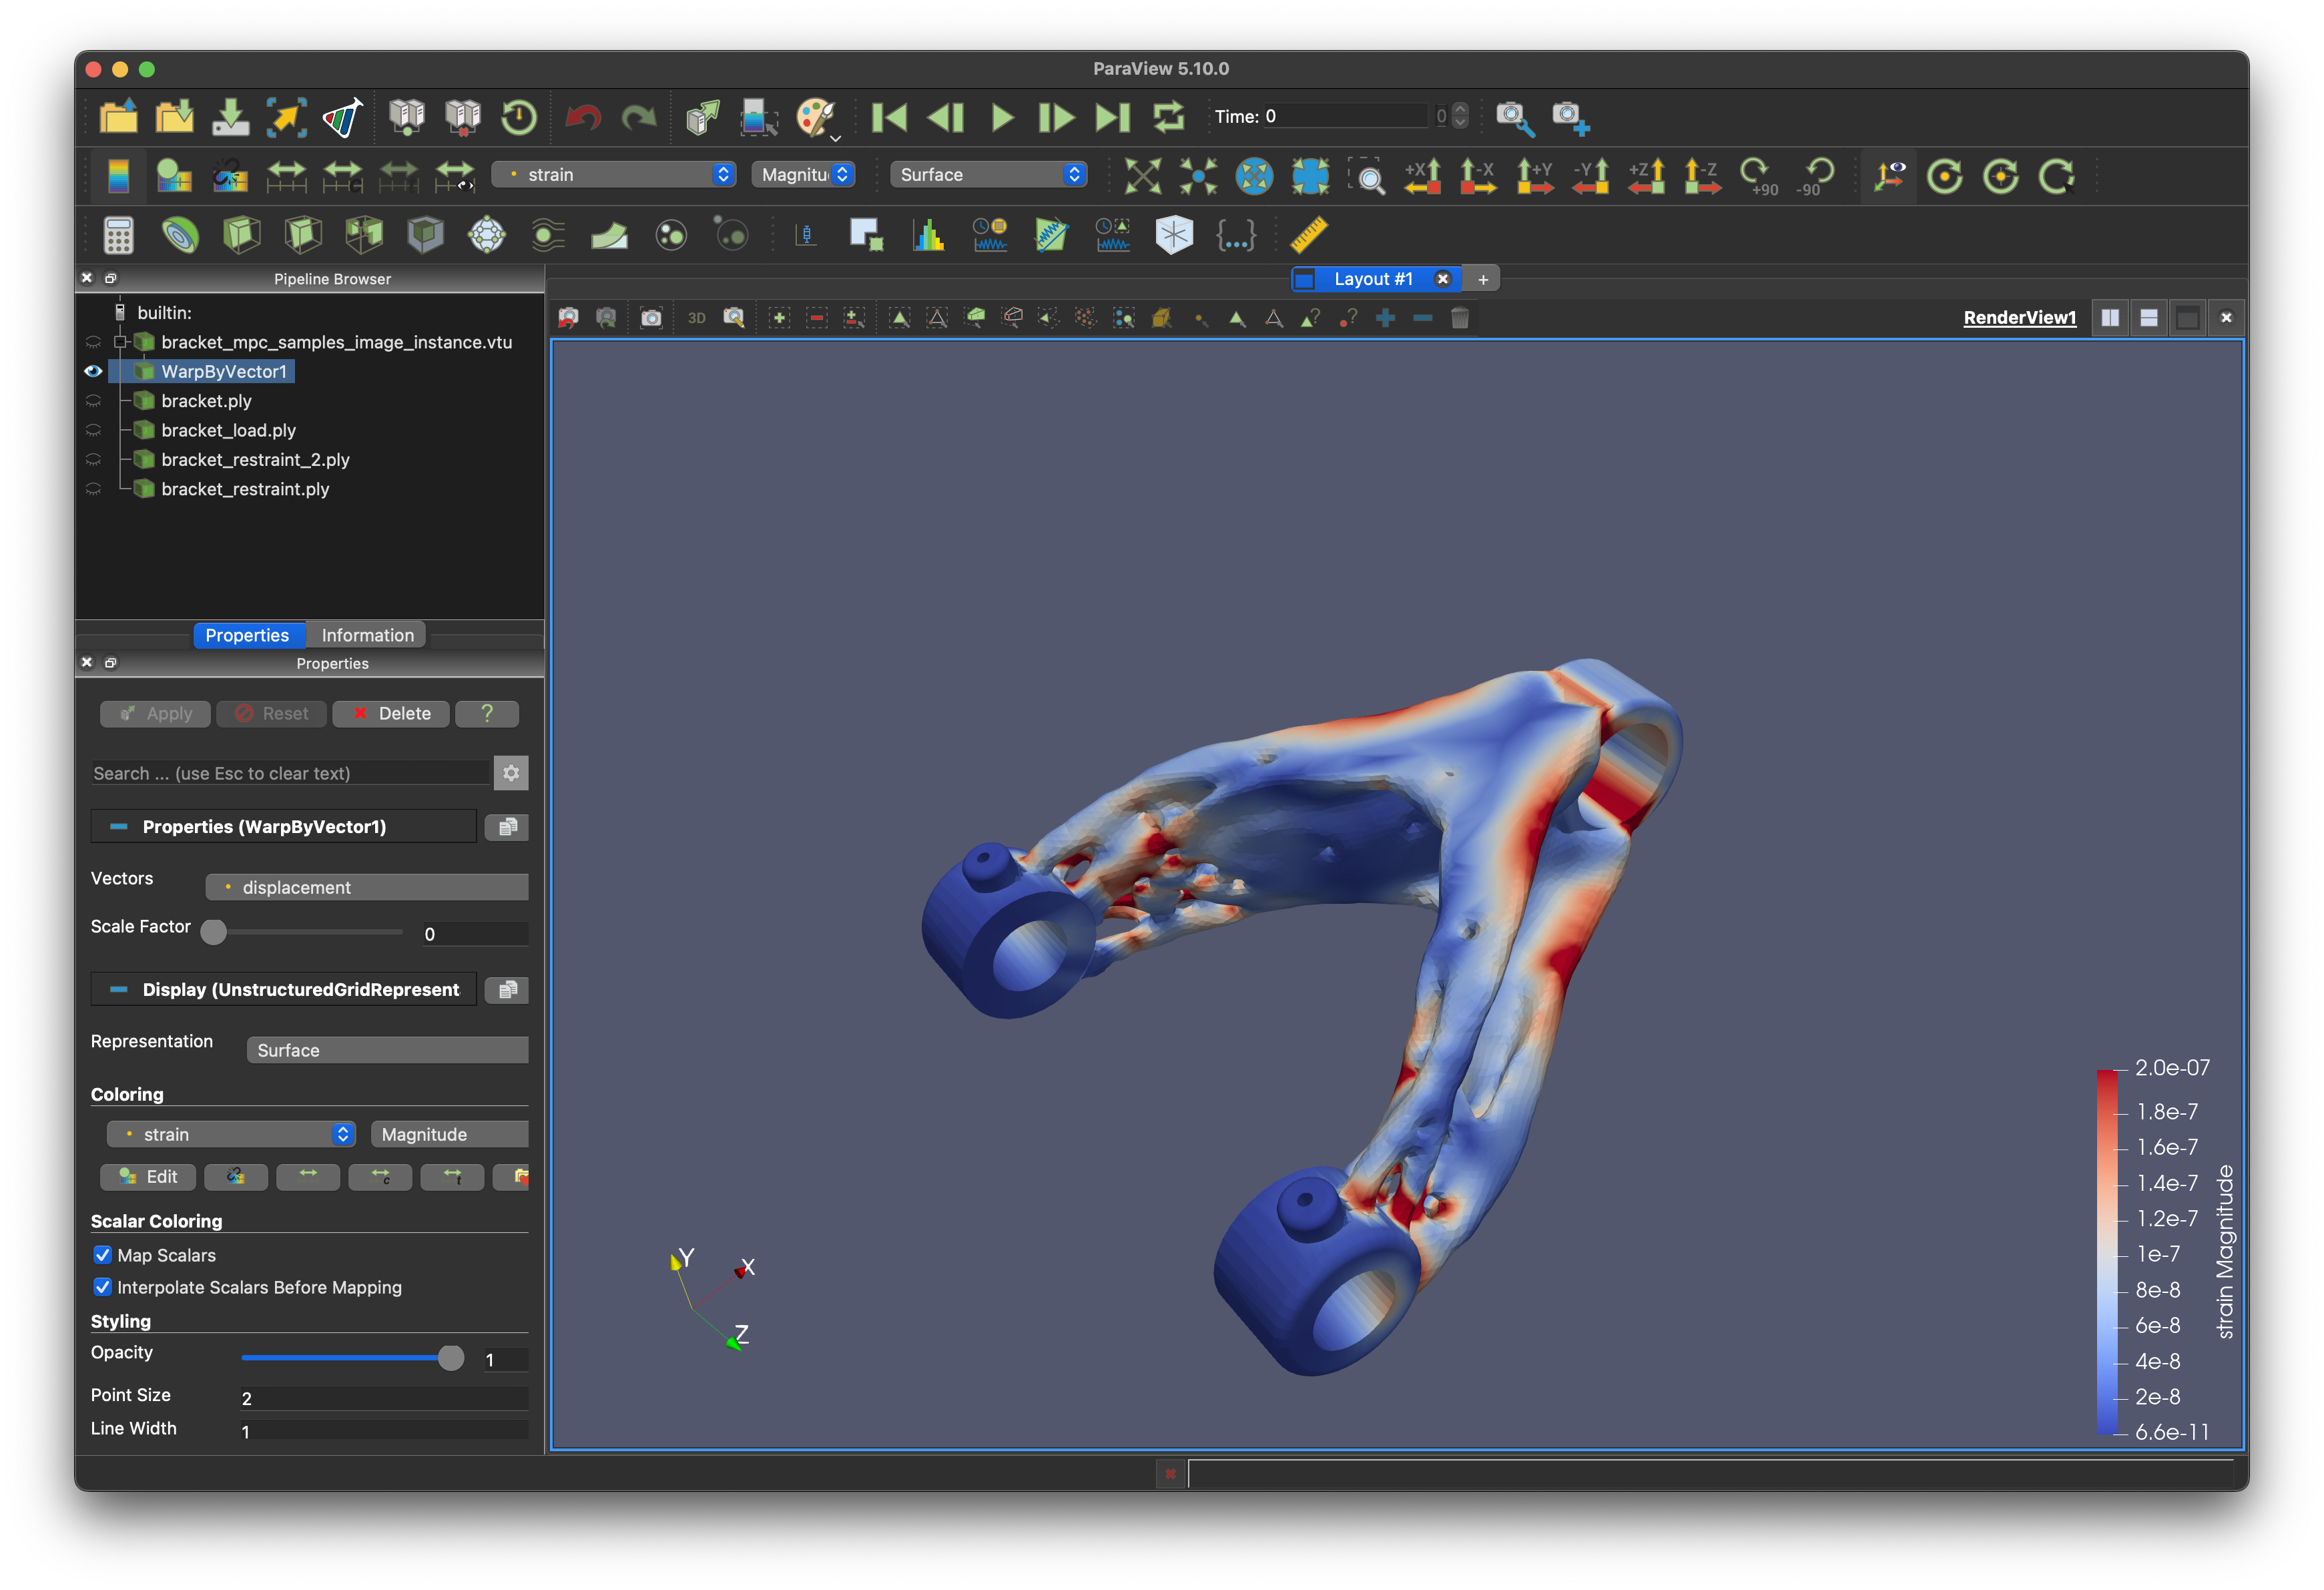
\includegraphics[width=0.7\linewidth]{bracket_demo.png}
  \end{center}
\end{frame}

\begin{frame}{FEA Workflow}
  \centering
  \begin{center}
    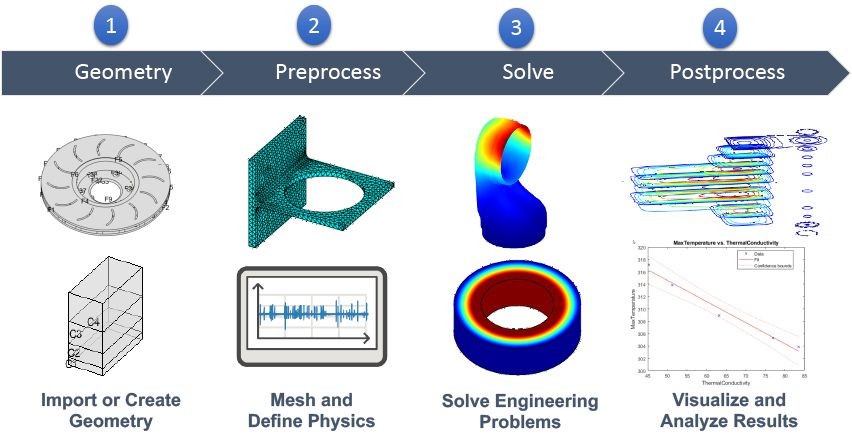
\includegraphics[width=0.7\linewidth]{fea_workflow.png}
  \end{center}
  \blfootnote{From \href{https://www.mathworks.com/discovery/finite-element-analysis.html}{MathWorks}}
\end{frame}
